%%%%%%%%%%%%%%%%%%%%%%%%%%%%%%%%%%%%%%%%%%%%%%%%%%%%%%%%%%%%%%%%%
% MUW Presentation
% LaTeX Template
% Version 1.0 (27/12/2016)
%
% License:
% CC BY-NC-SA 4.0 (http://creativecommons.org/licenses/by-nc-sa/3.0/)
%
% Created by:
% Nicolas Ballarini, CeMSIIS, Medical University of Vienna
% nicoballarini@gmail.com
% http://statistics.msi.meduniwien.ac.at/
%
% Customized for UAH by:
% David F. Barrero, Departamento de Automática, UAH
%%%%%%%%%%%%%%%%%%%%%%%%%%%%%%%%%%%%%%%%%%%%%%%%%%%%%%%%%%%%%%%%%

\documentclass[10pt,compress]{beamer} % Change 10pt to make fonts of a different size
\mode<presentation>

\usepackage[spanish]{babel}
\usepackage{fontspec}
\usepackage{tikz}
\usepackage{etoolbox}
\usepackage{xcolor}
\usepackage{xstring}
\usepackage{listings}
\usepackage{tikz}
\usetikzlibrary{matrix,chains,positioning,decorations.pathreplacing,arrows,shapes}

\usetheme{UAH}
\usecolortheme{UAH}
\setbeamertemplate{navigation symbols}{} 
\setbeamertemplate{caption}[numbered]

%%%%%%%%%%%%%%%%%%%%%%%%%%%%%%%%%%%%%%%%%%%%%%%%%%%%%%%%%%%%%%%%%
%% Presentation Info
\title[Scientific Programming]{Scientific Programming in Python}
\author{\asignatura\\\carrera}
\institute{}
\date{Departamento de Automática}
%%%%%%%%%%%%%%%%%%%%%%%%%%%%%%%%%%%%%%%%%%%%%%%%%%%%%%%%%%%%%%%%%


%%%%%%%%%%%%%%%%%%%%%%%%%%%%%%%%%%%%%%%%%%%%%%%%%%%%%%%%%%%%%%%%%
%% Descomentar para habilitar barra de navegación superior
\setNavigation
%%%%%%%%%%%%%%%%%%%%%%%%%%%%%%%%%%%%%%%%%%%%%%%%%%%%%%%%%%%%%%%%%

%%%%%%%%%%%%%%%%%%%%%%%%%%%%%%%%%%%%%%%%%%%%%%%%%%%%%%%%%%%%%%%%%
%% Configuración de logotipos en portada
%% Opacidad de los logotipos
\newcommand{\opacidad}{1}
%% Descomentar para habilitar logotipo en pié de página de portada
\renewcommand{\logoUno}{Images/isg.png}
%% Descomentar para habilitar logotipo en pié de página de portada
%\renewcommand{\logoDos}{Images/CCLogo.png}
%% Descomentar para habilitar logotipo en pié de página de portada
%\renewcommand{\logoTres}{Images/ALogo.png}
%% Descomentar para habilitar logotipo en pié de página de portada
%\renewcommand{\logoCuatro}{Images/ELogo.png}
%%%%%%%%%%%%%%%%%%%%%%%%%%%%%%%%%%%%%%%%%%%%%%%%%%%%%%%%%%%%%%%%%

%%%%%%%%%%%%%%%%%%%%%%%%%%%%%%%%%%%%%%%%%%%%%%%%%%%%%%%%%%%%%%%%%
%% FOOTLINE
%% Comment/Uncomment the following blocks to modify the footline
%% content in the body slides. 


%% Option A: Title and institute
\footlineA
%% Option B: Author and institute
%\footlineB
%% Option C: Title, Author and institute
%\footlineC
%%%%%%%%%%%%%%%%%%%%%%%%%%%%%%%%%%%%%%%%%%%%%%%%%%%%%%%%%%%%%%%%%

\begin{document}

%%%%%%%%%%%%%%%%%%%%%%%%%%%%%%%%%%%%%%%%%%%%%%%%%%%%%%%%%%%%%%%%%
% Use this block for a blue title slide with modified footline
{\titlepageBlue
    \begin{frame}
        \titlepage
    \end{frame}
}

\begin{frame}[plain]{}
	\begin{block}{Objectives}
		\begin{enumerate}
		\item Motivate the need of efficient matrix representations.
		\item Introduce some Python scientific tools.
		\item Handle data representations in Python.
		\item Basic data visualization with Python.
		\item Provide a background for scientific programming.
		\end{enumerate}
	\end{block}

   \begin{block}{Bibliography}
       Jake VanderPlas. \textit{Python Data Science Handbook}. Chapters 1, 2, 3 and 4. O'Reilly. \href{https://jakevdp.github.io/PythonDataScienceHandbook/}{(Link)}.
   \end{block}

\end{frame}

{
\disableNavigation{white}
\begin{frame}[shrink]{Table of Contents}
 \frametitle{Table of Contents}
 \tableofcontents
  % You might wish to add the option [pausesections]
\end{frame}
}

\section{Overview}

\subsection{Data Science}

\begin{frame}{Overview}{Data Science}
	\begin{figure}
		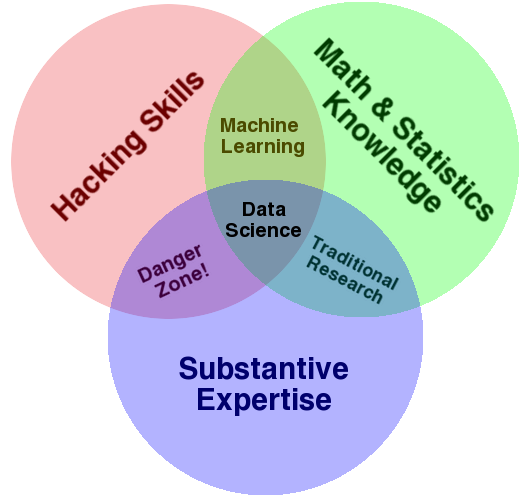
\includegraphics[scale=0.35]{figs/Data_Science_VD.png}	
	\end{figure}				
\end{frame}

\subsection{The data scientist toolkit}

\begin{frame}{Data Science}{The data scientist tookit (I)}
	Data science is about manipulating data
	\begin{itemize}
		\item Need of specialized tools
		\item Two main languajes: R and Python
	\end{itemize}
	Python is a general purpose programming language
	\begin{itemize}
		\item Easy integration 
		\item Huge ecosystem of packages and tools
	\end{itemize}
	Need of data-oriented tools
	\begin{itemize}
		\item Features provided by third-party tools
	\end{itemize}

\end{frame}

\begin{frame}{Data Science}{The data scientist tookit (II)}
   \begin{tabular}{cll}\hline
       \textbf{Tool}& \textbf{Type} & \textbf{Description}\\ \hline
	   \texttt{iPython} & Software & Advaced Python interpreter \\
	   \texttt{Jupiter} & Software & Python notebooks (Python interpreter) \\
	   \texttt{Numpy}   & Package  & Efficient array operations \\
	   \texttt{Pandas}  & Package  & Dataframe support \\
	   \texttt{Matplotlib} & Package & Data visualization \\
	   \texttt{Seaborn} & Package & Data visualization with dataframes \\
	   \texttt{Scikit-learn} & Package & AI/ML package for Python \\
	   \hline
   \end{tabular}
\end{frame}

\subsection{Anaconda}
\begin{frame}{Data Science}{Anaconda}
    \begin{columns}
 	   \column{.6\textwidth}
   All those tools are packaged in \texttt{Anaconda}
   \begin{itemize}
   		\item Python distribution for Data Science
	\end{itemize}

	Anaconda provides \texttt{Spyder}
	\begin{itemize}
		\item Python IDE designed for Data Science
	\end{itemize}

	Other tools provided by Anaconda
	\begin{itemize}
		\item Conda: Packages management tool
		\item TensorFlow: Deep Learning 
		\item Many others
	\end{itemize}

 		\column{.4\textwidth}
			
\includegraphics[width=0.6\textwidth]{figs/Anaconda_Logo.png} \\\bigskip
			
\includegraphics[width=0.6\textwidth]{figs/spyder.png}	
			%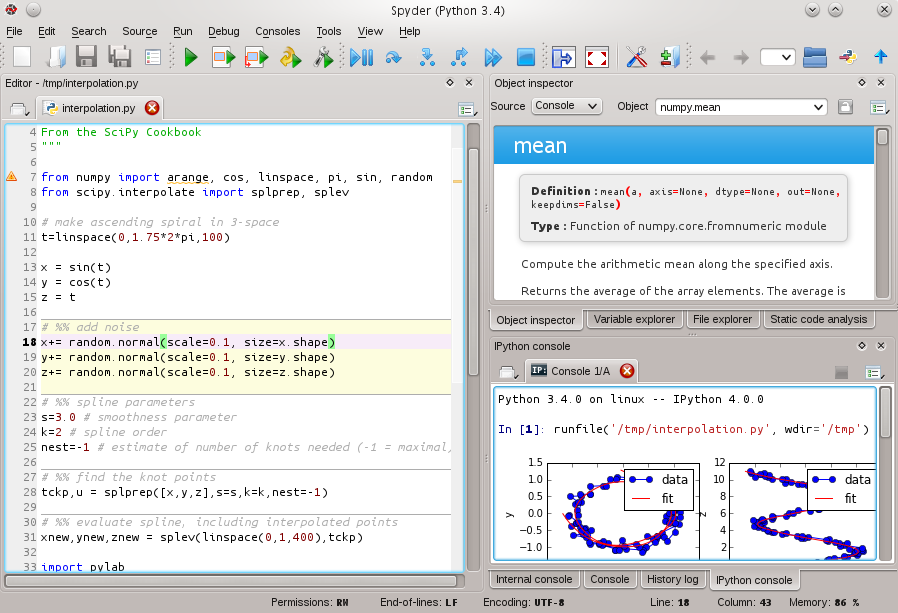
\includegraphics[width=0.6\textwidth]{figs/spyder-ide.png}	
	\end{columns}
\end{frame}

\subsection{Python IDEs for Data Science}
\begin{frame}{Data Science}{Python IDEs for Data Science (I)}
    \begin{columns}
 	   \column{.25\textwidth}
	   \centering \textbf{iPython}\\
	   iPython = Interactive Python
   		\begin{itemize}
		\item Extended funcionality
		\item Enhanced UI
		\item External editor
		\end{itemize}

		Running iPython:\\
		\texttt{\$ ipython}

 	   \column{.25\textwidth}
	   \centering \textbf{Jupyter}\\
		Python notebooks
	\begin{itemize}
		\item Web-based IDE
		\item Documentation
		\item Integration with GitHub
		\item Uses iPython
	\end{itemize}

		Running Jupyter:\\
		\texttt{\$ jupyter notebook}

		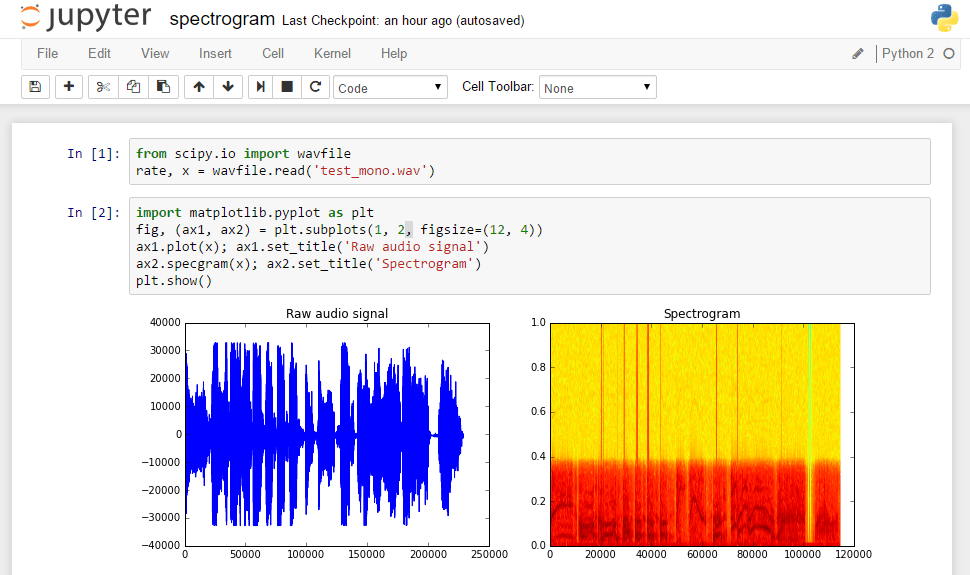
\includegraphics[width=0.8\textwidth]{figs/jupyter.png}	

 	\column{.25\textwidth}
	   \centering \textbf{Spyder}\\
		Matlab-like IDE

		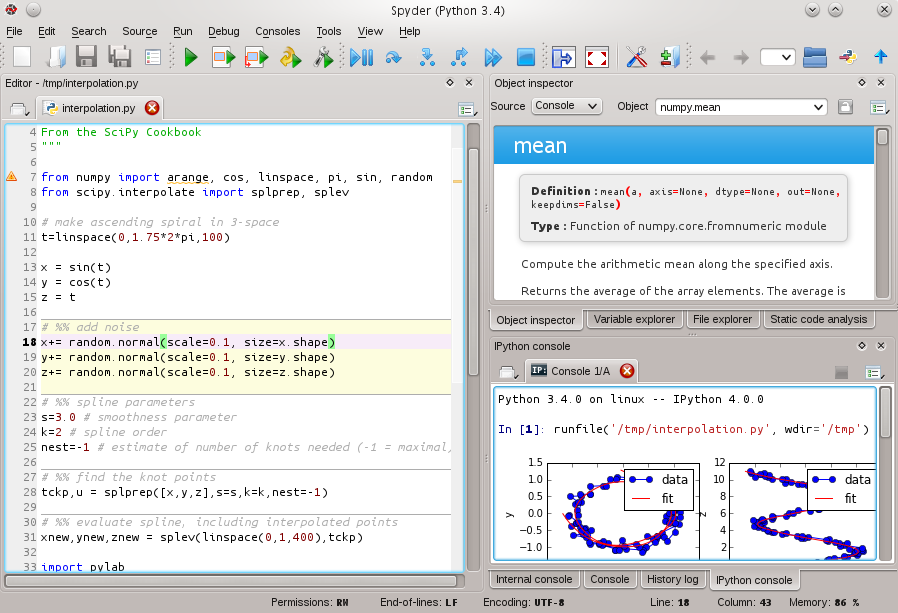
\includegraphics[width=0.8\textwidth]{figs/spyder-ide.png}	

 	\column{.25\textwidth}
	   \centering \textbf{Rodeo}\\
		Python version of RStudio
		\begin{itemize}
			\item Good for R developers
			\item Uses iPython
		\end{itemize}

		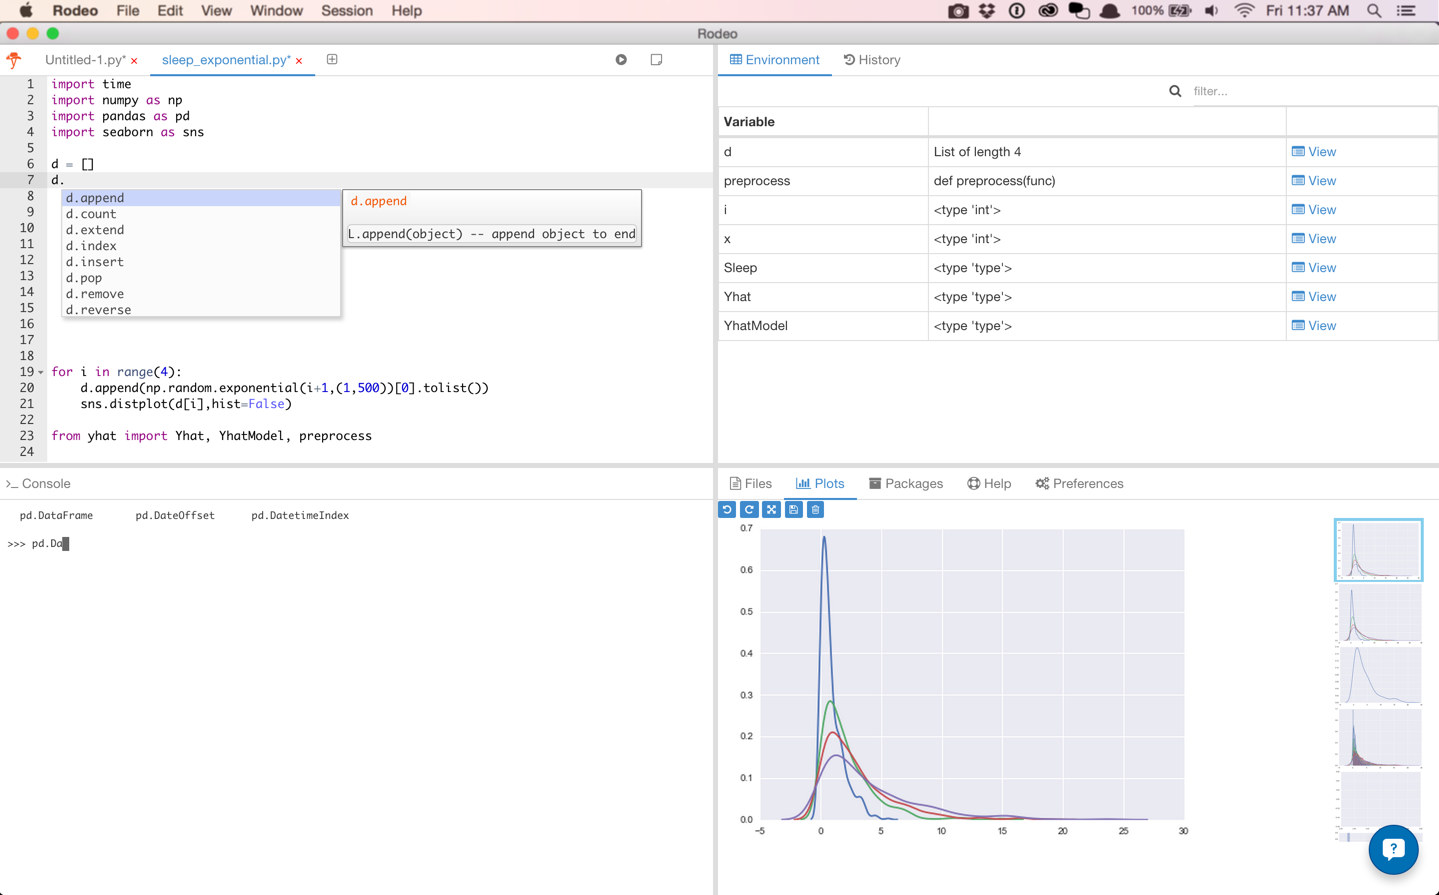
\includegraphics[width=0.8\textwidth]{figs/rodeo.png}	
	\end{columns}
\end{frame}

\begin{frame}{Data Science}{Python IDEs for Data Science (II)}
    \begin{block}{Exercises}
		Write a Python script that shows the multiplication table of the number 5 with each one of the following environments:
   		\begin{enumerate}
   		\item iPython + text editor of your choice.
		\item Jupiter. Bonus track: Publish the notebook in GitHub.
		\item Spyder.
		\item Rodeo.
		\end{enumerate}
	\end{block}
\end{frame}

\section{iPython}
\section{Numpy}
\section{Pandas}
\section{Matplotlib}
\section{Seaborn}

\begin{frame}{The data scientist working environment}
	\begin{block}{Imperative programming}
		Describes, by a set of instructions that change the \alert{program state}, \alert{how} the task should be implemented.  
  	\end{block}
  	\begin{itemize}
  		\item \textbf{Procedural}: organizes the program using collections of subroutines related by means of invocations (\textit{C, Python}).
  		\begin{itemize}
  			\item Example: \textit{The cooking process consists of 20 lines of code. When it is used, it only calls the function (1 line).} 
  		\end{itemize}
  		\item \textbf{Structural}: is based on nesting, loops, conditionals and subroutines. \texttt{GOTO} command is forbidden 				 \textit{(C, Pascal)}.
  		\begin{itemize}
  			\item Example: \textit{reviewing products of a shopping list and add the item X to the shopping if it is available.} 
  		\end{itemize}
  	\end{itemize}
\end{frame}

\begin{frame}{Programming paradigms types (III)}{}
	\begin{block}{Object-Oriented Programming}
		Evolves from imperative programming. It is based on \alert{objects} that allow express the \alert{characteristics} and \alert{behavior} in a closer way to real life (Java, Python, C++). 
  	\end{block}
  	\begin{itemize}
  		\item \textbf{Main characteristics}: abstraction, encapsulation, polymorphism, inheritance, modularity, etc.
		\item Example: \textit{a car has a set of properties (color, fuel type, model) and a functionality (speed up, shift gears, braking).} 
  	\end{itemize}
  	
\textit{\alert{There are many other paradigms such as Event-Driven programming, Concurrent, Reactive, Generic, etc.}}
\end{frame}

\begin{frame}{Programming paradigms types (IV)}{Classification}
	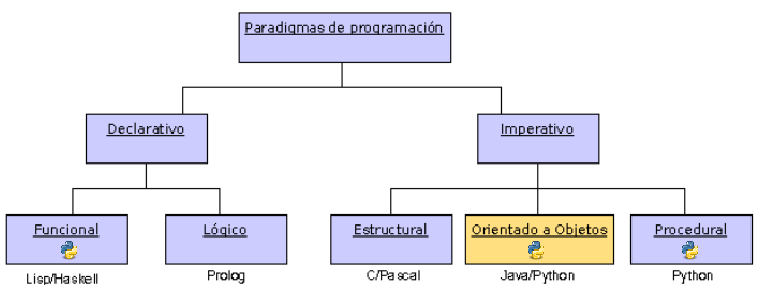
\includegraphics[scale=0.4]{figs/paradigmas}
	%\caption{http://www.computer.org/csdl/mags/it/2011/05/mit2011050030-abs.html}
	
	\centering\textit{\alert{Python supports the three major paradigms, although it stands out for the OOP and Imperative paradigms.}
}\end{frame}

\section[Object-Oriented Programming]{Object-Oriented Programming}

\subsection{Objectives}

\begin{frame}{Object-Oriented Programming}{Objectives}
\begin{itemize}
  	\item \textbf{Reusability}: Ability of software elements to serve for the construction of many different applications.
  	\item \textbf{Extensibility}: Ease of adapting software products to specification changes.
  	\item \textbf{Maintainability}: Amount of effort necessary for a product to maintain its normal functionality.   
  	\item \textbf{Usability}: Ease of using the tool.
  	\item \textbf{Robustness}: Ability of software systems to react appropriately to exceptional conditions.   
  	\item \textbf{Correction}: Ability of software products to perform their tasks accurately, as defined in their specifications.
  	\end{itemize} 	
\end{frame}

\subsection{Basic concepts}

\begin{frame}{Object-Oriented Programming}{Concepts (II)}
	\vfill\begin{block}{Atribute}
		Individual characteristics that determine the qualities of an object. 
  	\end{block}	
		\begin{figure}
			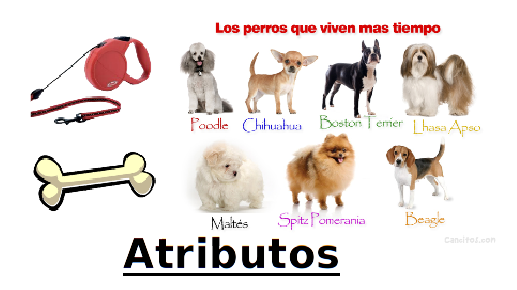
\includegraphics[scale=0.5]{figs/atributo}
		\end{figure}				
\end{frame}

\begin{frame}{Object-Oriented Programming}{Concepts (III)}
	\vfill\begin{block}{Method}
		 Function responsible for performing operations according to input parameters. 
  	\end{block}	
		\begin{figure}
			
\includegraphics[scale=0.5]{figs/metodo}
		\end{figure}				
\end{frame}

\begin{frame}{Object-Oriented Programming}{Concepts (IV)}
	\vfill\begin{block}{Object or instance}
		 Specific representation of a class, namely, a class member with their corresponding attributes.
  	\end{block}	  	
		\begin{figure}
			
\includegraphics[scale=0.5]{figs/instancia}
		\end{figure}				
\end{frame}

\begin{frame}{Object-Oriented Programming}{Concepts(V)}
	\begin{block}{Constructor}
		 Method called when an object is created. It allows the initialization of attributes. 
  	\end{block}	
		\begin{figure}
			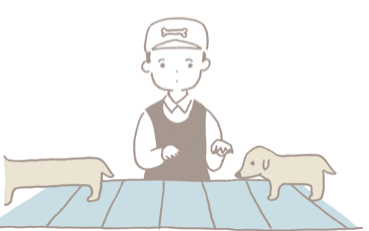
\includegraphics[scale=0.5]{figs/constructor}
		\end{figure}				
\end{frame}

\begin{frame}{Object-Oriented Programming}{Synthesizing OOP terminology}
    \begin{columns}
 	   \column{.6\textwidth}
 		  \begin{itemize}
			\item \small{Software objects mimics physical objects.} % un  individuo o ejemplar de una clase 
		   	\begin{itemize}
				\item \footnotesize{An object contains \textit{attributes} (state) and a \textit{behaviour}}. % behavior u operaciones
				\item \footnotesize{Example: A dog has a name (state) and may be a bit (behaviour).}
		  	\end{itemize}
		  %	\item Objects are grouped into classes.
		  	\item \small{A \alert{class} is a set of objects with common characteristics and behaviour.}
		  	\item \small{An \alert{object} is called an \alert{Instance} of a class.}
		  	% It can also be described as a pattern or template that is used to create objects.
			\item \textit{Members} of a class:
		    	\begin{itemize}
				\item \footnotesize{\alert{Properties}: Data describing an object.}
				\item \footnotesize{\alert{Methods}: What an object can do.}%Something that can be done to object. % o procedimiento perteneciente a un objeto.
					% modo en que se comunican los objetos entre síi. 
		  	    \end{itemize}
			% \item Property = Member, attribute, variable, etc.
		  \end{itemize}
 		\column{.4\textwidth}
	  	 	\begin{figure}[t]
			\begin{center}
			    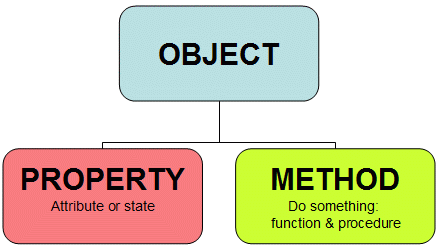
\includegraphics[width=0.97\linewidth]{figs/object2}\\
				\tiny{Source: http://www.teachitza.com/delphi/oop.htm}
			\end{center}
  	 		\end{figure}
    \end{columns}
\end{frame}


%Diapositiva del Main
%\begin{frame}{Programación Orientada a Objetos(I) - Definiciones (VI)}{}
%	\begin{block}{Main}
%		 \justifying Módulo principal muy util para la realización de pruebas. Permite incluir solamente los fragmentos de código que quieran ser probados.
%  	\end{block}	
%		\vspace{1cm}
%		\centering
\includegraphics[scale=0.1]{figs/main}
%\end{frame}


\subsection{Characteristics}

\begin{frame}{Characteristics}{Inheritance}
\vspace{-0.2cm}
	\begin{block}{Concept}
	Mechanism of \alert{reusing} code in OOP. Consists of generating child classes from other existing (\alert{super-class}) allowing the use and adaptation of the attributes and methods of the parent class to the child class. 
  	\end{block}	
\vspace{-0.2cm}
\begin{block}{}
\begin{itemize}
		\item \small{\textit{Superclass}: ``Father'' of a class.}
		\item \small{\textit{Subclass}: ``Child'' of a class.}
		\item \small{A subclass inherits all the fields and methods from its superclass.}
		\begin{itemize}
		\item \footnotesize \textit{Fields}: Variable that is part of an object.
		\end{itemize}
		\item \small{A subclass has \alert{one} superclass.}
		\item \small{A superclass has \alert{at least one} subclass.}
		\item \small{\textit{Class hierarchy}: A set of classes related by inheritance.}
\end{itemize}
	\end{block}
\end{frame}

\begin{frame}{Characteristics}{Inheritance (II)}

	\begin{block}{Types of inheritance}
	\begin{itemize}
		\item If the child class inherits from a single class is called \alert{single inheritance}.
		\item if it inherits from more classes is \alert{multiple inheritance}.
	\end{itemize}
	\end{block}
	\medskip
	   \textit{Python allows both; simple and multiple inheritance.}
\end{frame}

\begin{frame}{Characteristics}{Examples of simple inheritance (I)}
    \begin{columns}
    % cambiar figura poniendo fields y methods también
 	   \column{.40\textwidth}
	    \centering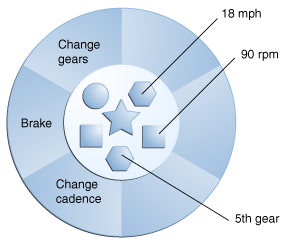
\includegraphics[width=0.9\linewidth]{figs/concepts-bicycleObject2}
	  
	    \column{.60\textwidth}
	  \centering 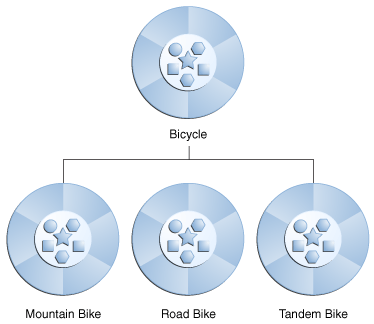
\includegraphics[width=0.9\linewidth]{figs/concepts-bikeHierarchy2}\\
	
    \end{columns}
    \bigskip
	\centering \tiny{Source: http://docs.oracle.com/javase/tutorial/java/concepts/object.html}\\
	\centering \tiny{Source: http://docs.oracle.com/javase/tutorial/java/concepts/inheritance.html}\\
\end{frame}

\begin{frame}{Characteristics}{Examples of simple inheritance (II)}
	\begin{figure}
		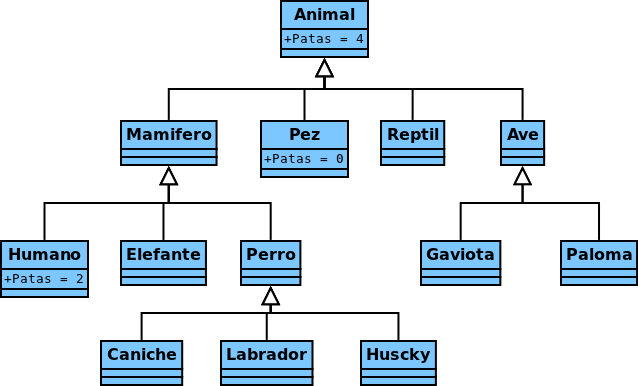
\includegraphics[scale=0.33]{figs/herencia1}
		\caption{{\scriptsize Example of simple Inheritance in OOP. Obtained from: \url{http://android.scenebeta.com}}}
	\end{figure}
\end{frame}



\begin{frame}{Characteristics}{Multiple Inheritance}
	\begin{figure}
		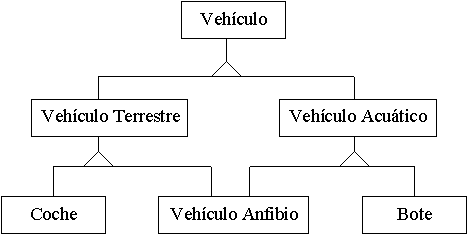
\includegraphics[scale=0.5]{figs/herencia2}
		\caption{{\scriptsize Example of multiple Inheritance in OOP. Obtained from: \url{http://www.avizora.com}}}
	\end{figure}
\end{frame}

\begin{frame}{Characteristics}{Polymorphism (I)}
\vspace{-0.2cm}
	\begin{block}{Polymorphism}
		Mechanism of object-oriented programming that allows to invoke a method whose implementation will depend on the object that does it.
  	\end{block}	
% TIPOS DE POLIMORFISMO
%		\begin{itemize}
%			\item \justifying\textbf{Polimorfismo de sobrecarga}: mismo nombre y tipos de 						  datos en diferentes clases.
%			\item \justifying\textbf{Polimorfismo paramétrico}: mismo nombre diferentes 							  tipos de datos. 
%			\item \justifying\textbf{Polimorfismo de subtipado}: Permite invocar un método 						  de una clase especializada a partir de la clase padre.
%		\end{itemize}
	\begin{figure}
	  \vspace{-0.2cm}
		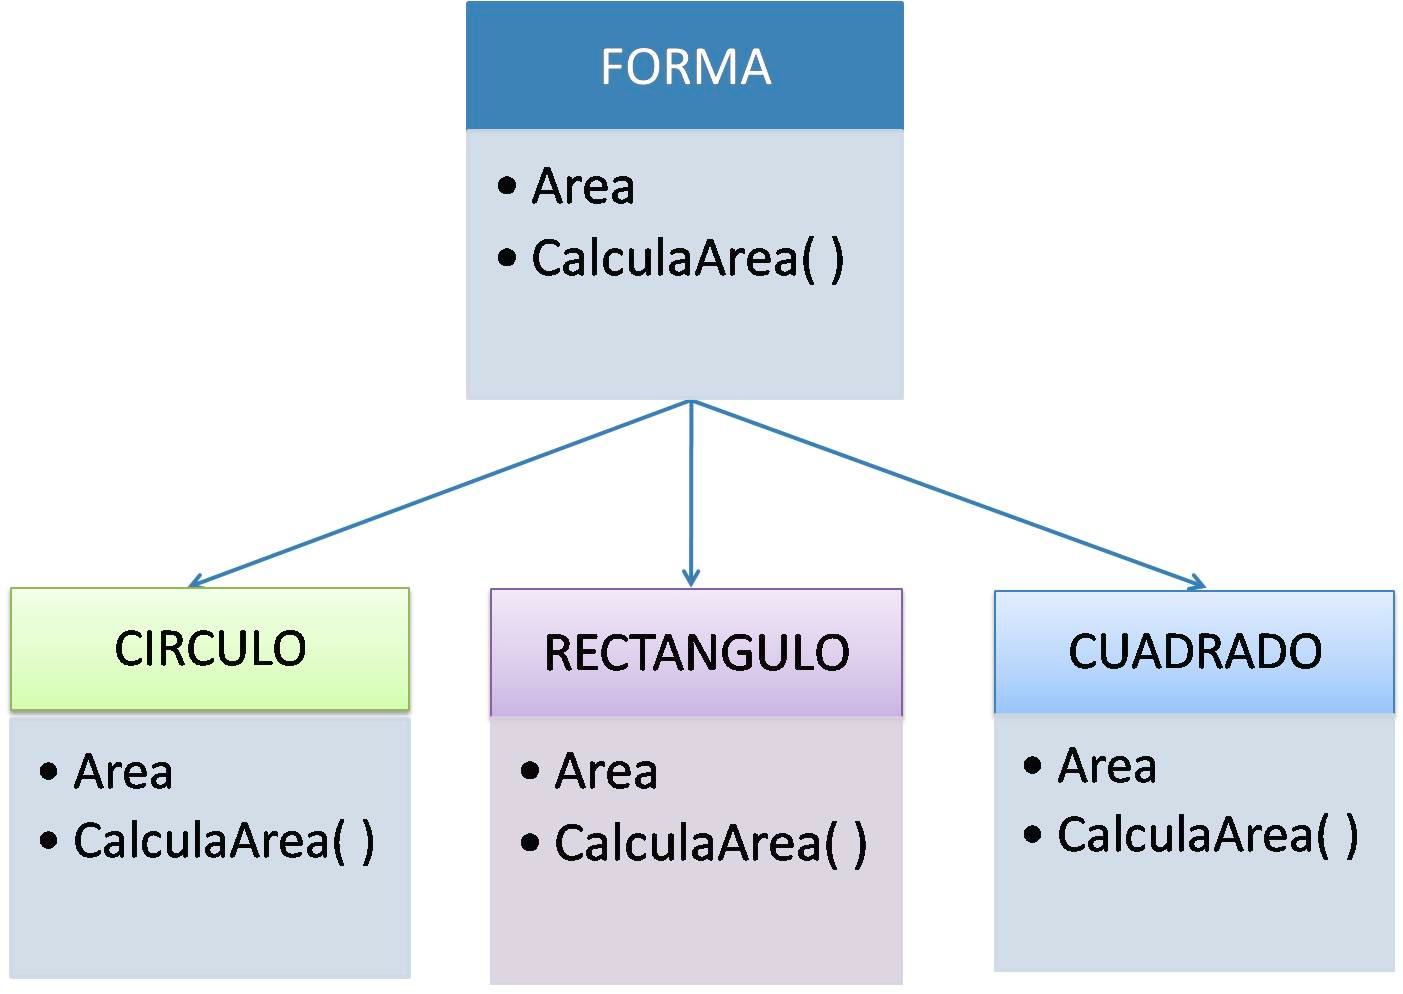
\includegraphics[width=4.6cm]{figs/polimorfismo1}
		\vspace{-0.2cm}
		\caption{\scriptsize{Example of polymorphism. Obtained from: \url{http://virtual.uaeh.edu.mx}}}
	\end{figure}
\end{frame}

\begin{frame}{Characteristics}{Polymorphism (II)}
	\begin{figure}
		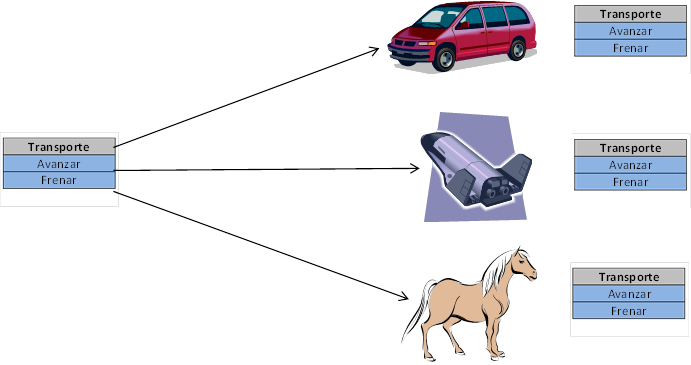
\includegraphics[scale=0.57]{figs/polimorfismo2}
		\vspace{-0.1cm}
		\caption{{\scriptsize Example of polymorphism. Obtained from: \url{http://datateca.unad.edu.co}}}
	\end{figure}
\end{frame}


\begin{frame}{Characteristics}{Abstraction and encapsulation (I)}
	\begin{block}{Abstraction}
		Mechanism that allows the isolation of the not relevant information to a level of knowledge.
  	\end{block}	
	
	\begin{itemize}
		\item \textit{A driver does not need to know how the carburetor works.} 
		\item \textit{To talk on the phone does not need to know how the voice is transferred.} 
		\item \textit{To use a computer do not need to know the internal composition of their materials}. 							  
		
%		\vfill\item \textit{\alert{En Python no existen de manera nativa las clases 					abstractas pero si mediante el módulo ABC \cite{PythonTeam}.}}
	\end{itemize}
\end{frame}

\begin{frame}{Characteristics}{Abstraction and encapsulation (II)}
	\begin{block}{Encapsulation}
		Mechanism use to provide an access level to methods and attributes for avoiding unexpected state changes. This mechanism is used to limit the visibility of the attributes and to create methods controlling them (\texttt{set()} y \texttt{get()}).
  	\end{block}	
	
The most common access levels are:
	
	\begin{itemize}
		\item \textbf{public}: visible for everyone  [default level in Python].
		\item \textbf{private}: visible for the creator class [start with a double underscore and does not end in the same manner].
		\item \textbf{protected}: visible for the creator class and its descendents \alert{[not exist in Python]}. 
	\end{itemize}
\end{frame}

\begin{frame}{Characteristics}{Abstraction and encapsulation (III). Example 1}
	\begin{figure}
		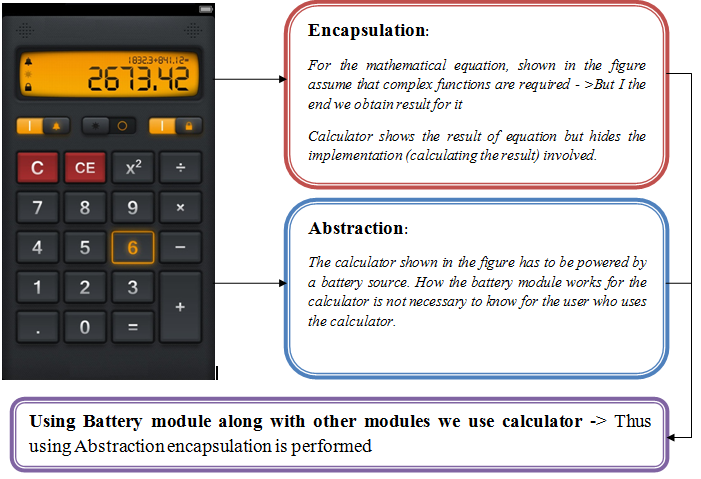
\includegraphics[scale=0.4]{figs/abstraccion1}
		\caption{{\scriptsize Example of abstraction and encapsulation.Obtained from: \url{https://binalparekh.wordpress.com}}}
	\end{figure}
\end{frame}

\begin{frame}{Characteristics(III)}{Abstraction and encapsulation (IV). Example 2}
	\begin{figure}
		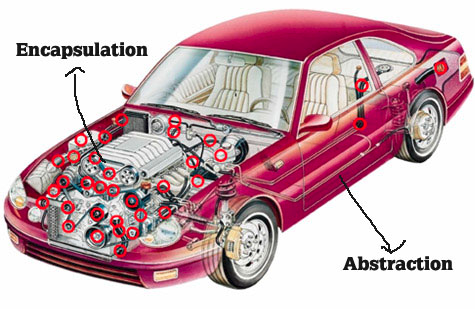
\includegraphics[scale=0.45]{figs/abstraccion2}
		\caption{{\scriptsize Example of abstraction and encapsulation. Obtained from: \url{http://www.onlinebuff.com}}}
	\end{figure}
\end{frame}

\section{Classes in Python}
   \subsection{Sintax}
%Sintaxis básica
%\begin{frame}{Nomeclatura de Python}{Sintaxis(I)}
%	\begin{itemize}
%		\item \justifying \textbf{Impresión por pantalla}: \texttt{print}. Por defecto solo admite la codificación inglesa (sin tildes ni ñ). 
%		\begin{itemize}
%			\item Para que las admita, se escribe antes: \# -*- coding: utf-8 -*-
%			\item Para imprimir texto se escribe entre comillas dobles.
%		\end{itemize}
%		\item \justifying\textbf{Indentación}: Python utiliza espacios o tabulaciones para definir los distintos niveles en el código, por lo tanto si un 													   fragmento se encuentra a la derecha del superior indica que está contenido en la instrucción anterior.
%		\item \justifying \textbf{Comentarios}: Comienzan con \#.
%	\end{itemize}
%    \begin{columns}
% 	   \column{0.8\textwidth}
%			\begin{block}{holaMundo.py}
%			\vspace{-0.3cm} 
%				\lstinputlisting[basicstyle=\ttfamily\scriptsize]{code/holaMundo.py} % contar elementos
%			\end{block}
%	\end{columns}			

%\end{frame}

%\begin{frame}{Nomeclatura de Python}{Sintaxis(II)}
%	\begin{itemize}
%		\item \justifying \textbf{Asignación}: Se expresa mediante un igual.
%		\item \justifying \textbf{Atributo}: sustantivo expresado con minúscula.
%		\item \justifying \textbf{Condiciones}: \texttt{if/elif/else + condición:}. Permiten expresar que hacer si se satisface o no una condición. Para 														expresar una condición de igualdad se utiliza \texttt{==}
%    \begin{columns}
% 	   \column{0.8\textwidth}
%			\begin{block}{semaforo.py}
%			\vspace{-0.3cm} 
%				\lstinputlisting[basicstyle=\ttfamily\scriptsize]{code/semaforo.py} % contar elementos
%			\end{block}
%	\end{columns}			
%	\end{itemize}
%\end{frame}


%\begin{frame}{Nomeclatura de Python}{Sintaxis(III)}
%	\begin{itemize}
%		\item \justifying \textbf{Estructuras iterativas}: \texttt{while/for + condición:}. Permiten expresar el mismo código mientras se cumpla la condición.	
%	\end{itemize}
%    \begin{columns}
% 	   \column{0.8\textwidth}
%			\begin{block}{provincias.py}
%			\vspace{-0.3cm} 
%				\lstinputlisting[basicstyle=\ttfamily\scriptsize]{code/provincias.py} % contar elementos
%			\end{block}
%	\end{columns}				 
%\end{frame}


\begin{frame}{Classes in Python}{Syntax (I)}
\vspace{-0.2cm}
\begin{itemize}			
		\item \small{\textbf{Class}: Start with the word \alert{class} followed by class name written in \alert{capital letter} and a colon [Substantives].}
		\item \small{\textbf{Attributes}: A lowercase noun.}
		\begin{itemize}
		\item \footnotesize{There is no need to declare attributes.}
		\end{itemize}
		
		\item \small{\textbf{Inherited class}: Similar to a class but the class name followed by the class father in brackets.}
		\item \small{\textbf{Instance}: Object in lower case followed by the class assignment.}
			\vspace{-0.2cm} 
  	   \begin{columns}
 	   \column{0.8\textwidth}
			\begin{block}{\small{coche.py}}
			\vspace{-0.3cm} 
				\lstinputlisting[basicstyle=\ttfamily\scriptsize]{code/coche.py} % contar elementos
				\vspace{-0.2cm} 
			\end{block}
	\end{columns}		
\end{itemize}			
\end{frame}

\begin{frame}{Classes in Python}{Syntax (II)}
\begin{itemize}
		\item \textbf{Method}: Start with the word \alert{def}, and later the method, a verb, in lower case is written. Next, the parameter in brackets and a colon (\texttt{print\_name()}).
   \begin{itemize}
   \item Methods receive automatically a reference to the object (usually named \texttt{self}).
   \end{itemize}
		\item \textbf{Constructor}: Method whose name is \texttt{\_\_init\_\_()}, the first attribute is \texttt{self} and then the class attributes are written.

		\item \textbf{main}: Method defined with \texttt{def main():}. In it, the wished commands are specified and after it, an exit condition is created. The \texttt{sys} module  is required to be imported at the beginning. 
		\item All methods and attributes are public.
			\begin{itemize}
				\item By convention, private members begin with double underscore (\texttt{\_\_varName}, \texttt{\_\_method\_name()})
			\end{itemize}
\end{itemize}			
\end{frame}


\begin{frame}{Classes in Python}{Syntax (III). Example 1}
    \begin{columns}
 	   \column{0.8\textwidth}
			\begin{block}{main.py}
			\vspace{-0.3cm} 
				\lstinputlisting[basicstyle=\ttfamily\scriptsize]{code/main.py} % contar elementos
			\end{block}
	\end{columns}				 	
\end{frame}

\begin{frame}{Classes in Python}{Syntax (IV). Example 2}
\vspace{-0.2cm}
    \begin{columns}
 	   \column{0.8\textwidth}
			\begin{block}{bicicleta.py}
			\vspace{-0.3cm} 
				\lstinputlisting[basicstyle=\ttfamily\scriptsize]{code/bicicleta.py} % contar elementos
			\vspace{-0.3cm} 
			\end{block}
	\end{columns}				 	
\end{frame}

\begin{frame}{Classes in Python}{Syntax (V). Example 3}
	\vspace{-0.2cm}
	\begin{block}{Time.py}
	\vspace{-0.3cm}
		\lstinputlisting{code/Time.py}
	\vspace{-0.3cm} 
	\end{block}
\end{frame}

\subsection{Class objects}
\begin{frame}[fragile]{Classes in Python}{Class objects}
	\centering {Two operations on classes}
    \begin{columns}
 	   \column{.50\textwidth}
	   		\begin{block}{Attribute references}
			Accesses an attribute value\\
			Standard dot syntax\\
			\bigskip
			\centering{\texttt{obj.name}}\\
	   		\end{block}
	   		\begin{exampleblock}{Example}
\begin{verbatim}
time.hour = 4
print(time.hour)
hour = time.hour
\end{verbatim}
	   		\end{exampleblock}

 	   \column{.50\textwidth}
	   		\begin{block}{Instantiation}
			Creates a new object\\
			Standard functional notation\\
			\bigskip
			\centering{\texttt{x = MyClass()}}\\
	   		\end{block}
	   		\begin{exampleblock}{Example}
\begin{verbatim}
time = Time()
\end{verbatim}
	   		\end{exampleblock}
	\end{columns}
\end{frame}

\subsection{Constructors}
\begin{frame}{Constructors (I)}
		Instantiation creates empty objects
		\begin{itemize}
			\item We usually need to initialize attributes
			\item Initialization operations
		\end{itemize}
		\alert{Constructor}: Method called when an object is created
		\begin{itemize}
			\item In Python, it is the \texttt{\_\_init\_\_()}
			\item A constructor can get arguments
		\end{itemize}
\end{frame}

\begin{frame}[plain]{Constructors (II)}
	\vspace{-0.3cm}
	\begin{block}{Time.py with constructor}
	\vspace{-0.3cm}
		\lstinputlisting{code/Time2.py}
	\end{block}
\end{frame}

\subsection{More about methods}

\begin{frame}{Other special methods}
In addition to special method \texttt{\_\_init\_\_}, there are several others, including:\\
	\begin{block}{}
		\vspace{-0.15cm}
		\begin{itemize}
		\item \footnotesize{\texttt{\_\_str\_\_(self)} It should return a string with \texttt{self} information.  When \texttt{print()} is invoked with the object, if the method \texttt{\_\_str\_\_()} is defined, Python shows the result of running this method on the object.}
		\item \footnotesize{\texttt{\_\_len\_\_(self)} It should return the length or ``size'' of object (number of elements if is a \textit{set} or \textit{queue}).}
		\item \footnotesize{\texttt{\_\_add\_\_(self, otro\_obj)} It allows to apply the addition operator (+) to objects of the class in which it is defined.}
		\item \footnotesize{\texttt{\_\_mul\_\_(self, otro\_obj)} It allows to apply the multiplication operator (*) to objects of the class in which it is defined.}
		\item \footnotesize{\texttt{\_\_comp\_\_(self, otro\_obj)} It allows to apply the comparison operators (<, >, <=, >=, ==, !=) to objects of the class in which it is defined. It should return 0 if they are equal, -1 if \texttt {self} is smaller than \texttt{other\_obj} and 1 if \texttt{self} is greater than \texttt{other\_obj}.}
		\end{itemize}
		\vspace{-0.2cm}
	\end{block}	
\end{frame}


\begin{frame}[shrink]{Overriding methods (I)}
	Often we need to adapt an inheritanced method: \alert{Overriding}

	\begin{block}{Overriding example}
		\vspace{-0.2cm}
		\lstinputlisting{code/Overriding.py}
		\vspace{-0.2cm}
	\end{block}
\end{frame}
	
\begin{frame}{Overriding methods (II)}
		Still possible to get superclass' method with \texttt{super()}

	\begin{block}{\texttt{super()} example}
		\vspace{-0.2cm}
		\lstinputlisting{code/Overriding2.py}
		\vspace{-0.2cm}
	\end{block}
\end{frame}

\subsection{Solved exercises}

\begin{frame}{Exercise statement}{\texttt{Animal} class}
	\begin{enumerate}
		\item Create the \texttt{animal} class. 
		\item Create the constructor. The class will have the attributes \texttt{tipo} and \texttt{patas}.
		%con las variables tipo de animal y número de 		patas.
		\item Create the get methods from both attributes which receive like own parameter the animal through \texttt{self} and return respectively the \texttt{tipo} and \texttt{patas}. 
		\item Create two instances of animals using the constructor.
		\item Print the attributes of both instances.
	\end{enumerate}	
\end{frame}

\begin{frame}{Solved exercise}{\texttt{Animal} class}
	\vspace{-0.2cm}
    \begin{columns}
 	   \column{0.8\textwidth}
			\begin{block}{animales.py}
			\vspace{-0.3cm} 
				\lstinputlisting[basicstyle=\ttfamily\scriptsize]{code/animales.py} % contar elementos
			\vspace{-0.3cm} 
			\end{block}
	\end{columns}
\end{frame}

\begin{frame}{Solved exercise}{\texttt{Animal} class}
	\begin{enumerate}
		\item Create a \texttt{gato} class in the same file which inherits from the \texttt{animal} class. 
		\item Create the constructor and add the \texttt{sonido} attribute. 
		\item Create the method \texttt{maullar} which prints the sound MIAU. 
		\item Create a instance and check the methods.
	\end{enumerate}	
\end{frame}

\begin{frame}{Solved exercise}{Class \texttt{Animals}}
	\vspace{-0.4cm}
    \begin{columns}
 	   \column{0.8\textwidth}
			\begin{block}{animales.py}
			\vspace{-0.3cm} 
				\lstinputlisting[basicstyle=\ttfamily\scriptsize]{code/gato.py} % contar elementos
			\vspace{-0.3cm} 
			\end{block}
	\end{columns}
\end{frame}
% añadir otro ejemplo de clases GIS , pickle de clases y más referencias
\begin{frame}{Exercise statement}{Class \texttt{Parcela}}
	\begin{enumerate}
		\item Create a script containing the class \texttt{Parcela}. 
		\item Create the constructor. The class will have the attributes \texttt{uso\_suelo} and \texttt{valor}.
		%con las variables tipo de animal y número de 		patas.
		\item Create the \texttt{valoracion} method to calculate the tax associated with the parcel as follows: 
		\begin{itemize}
		\item For single-family residential: \textit{tasa = 0.05 * valor}
		\item For multifamily residential: \textit{tasa = 0.04 * valor}
		\item For all other land uses: \textit{tasa = 0.02 * valor}
		\end{itemize}
		\item Use the class from another \textit{script} named \texttt{tasaparcela.py} which you create una instance of \texttt{Parcela} named \texttt{miparcela} using the constructor.
		\item Print the attribute  \texttt{uso\_suelo} of the instance.
		\item Use the method \texttt{valoracion} of \texttt{Parcel} to calculate the assessment of \texttt{miparcela}.
	\end{enumerate}	
\end{frame}

\begin{frame}{Solved exercise}{Class \texttt{Parcela}}
	\vspace{-0.26cm}
  %  \begin{columns}
 %	   \column{0.8\textwidth}
			\begin{block}{claseparcela.py}
			\vspace{-0.3cm} 
				\lstinputlisting[basicstyle=\ttfamily\scriptsize]{code/claseparcela.py} % contar elementos
			\vspace{-0.3cm} 
			\end{block}
%	\end{columns}
%	\tiny{\href{http://esripress.esri.com/display/index.cfm?fuseaction=display&websiteID=276&moduleID=0}{Source}}
\end{frame}

\begin{frame}{Solved exercise}{Use of \texttt{Parcela}}
	\vspace{-0.4cm}
    \begin{columns}
 	   \column{0.8\textwidth}
			\begin{block}{tasaparcela.py}
			\vspace{-0.3cm} 
				\lstinputlisting[basicstyle=\ttfamily\scriptsize]{code/tasaparcela.py} % contar elementos
			\vspace{-0.3cm} 
			\end{block}
	\end{columns}
		\tiny{\href{http://esripress.esri.com/display/index.cfm?fuseaction=display&websiteID=276&moduleID=0}{Source}}
\end{frame}

\begin{frame}[plain]{Solved exercise. Serializando objetos \texttt{Parcela}}{}
%	\vspace{-0.4cm}
  %  \begin{columns}
 %	   \column{0.8\textwidth}
			\begin{block}{\footnotesize{tasaparcela\_pickle.py}}
			\vspace{-0.2cm} 
				\lstinputlisting[basicstyle=\ttfamily\scriptsize]{code/tasaparcela_pickle.py} % contar elementos
			\vspace{-0.2cm} 
			\end{block}
%	\end{columns}
	
\end{frame}

\subsection{Approach to a final problem}
\begin{frame}{Exercise statement}{\texttt{Rio} class}
\vspace{-0.24cm}
	\begin{enumerate}
		\item Create the \texttt{Rio} class. 
		\item Create the constructor and add the \texttt{nombre} and \texttt{longitud} attributes.
		\item \texttt{Longitud} attribute must be private.
		\item Create the \texttt{setLongitud} method which receives self and \texttt{longitudR} and allows the set of any value for \texttt{longitud}.
		\item Create the \texttt{getNombre} method which obtains the name of the river.
		\item Create the \texttt{getLongitud} method which obtains the river length.		 
		\item Create an instance and check the methods.
		\item Try to do an assignment of \texttt{rio.nombre} and other assignment with  \texttt{rio.longitud} What happen? It is correct  to invoke the method named \texttt{rio.getLongitud()} out of the classes? How do you explain that?
	\end{enumerate}	
\end{frame}

\begin{frame}{Exercise statement}{Establishment of hierarchies from \texttt{Rio} class}
\vspace{-0.24cm}
	\begin{enumerate}
		\item Add to the \texttt{Rio} class the attribute \texttt{caudal} and the method \texttt{trasvasar} which receives two rivers and transfers 5 liters from the first to the second.
		\item Create the \texttt{Afluente} class which inherits from \texttt{Rio}.		
		\item Create the method \texttt{\_\_init\_\_} of \texttt{Afluente} which initializes its \texttt{nombre} and \texttt{longitud} and, also,  \texttt{afluenteDeRio}, new attribute initialized with the name of the river which the affluent starts.
		\item Is there any polymorphism in this sample?
		\item Create the main and exit condition and try it. Does the main position affect to the application? 
		\item Experiment now with conditions and iterative structures limiting when a river can transfer water or try to do some transfer at the same time.

	\end{enumerate}	
\end{frame}

\begin{frame}{Y más\dots}{}
Aprende más: \cite{Dusty}
\end{frame}


\appendix
\section<Bibliographic references>*{\appendixname}
\subsection<Bibliographic references>*{Bibliographic references}

\begin{frame}[t, allowframebreaks, plain]
  \frametitle<presentation>{Bibliographic references}

  \begin{thebibliography}{2}
  
  \beamertemplatebookbibitems
  % libro
  
   \bibitem{Dpto-CCIA-U.A}[1]
    Lenguajes de programacion, capítulo 1.
    \newblock \emph{Lenguajes de programacion}.
  \newblock \url{http://rua.ua.es/dspace/bitstream/10045/4030/1/tema01.pdf}
  
  % libro
   \bibitem{Downey}[2]
   Downey, A and Elkner, J and MEYER, C.
    \newblock \emph{Aprenda a Pensar como un Programador con Python, capitulos 14 y 16}.
    \newblock Green Tea Press, 2002.
    
    \bibitem{vanRossum}[3]
    G. van Rossum, Jr. Fred L. Drake.
    \newblock \emph{Python Tutorial Release 3.2.3, chapter 9}.
    \newblock Python Software Foundation, 2012. 
    
     \bibitem{Dusty}[4]
    Dusty Phillips
    \newblock \emph{Python 3 Object Oriented Programming}.
    \newblock Packt Publishing, 2010.
   
   % \bibitem{Swaroop}[Swaroop, 2008]
   %  C. H. Swaroop.
   % \newblock \emph{A byte of Python}.
   % \newblock Creative Commons Atribucion-NoComercial 3.0, 2008.
  \end{thebibliography}
\end{frame}

\end{document}
